\documentclass[12pt]{exam}
\newcommand{\hwnumber}{10}
\newcommand{\hwname}{Lights Out}
\newcommand{\duedate}{\formatdate{18}{04}{\YEAR} by \progDueTime}

\usepackage{../misc/latex/edition}  % Course semester
\usepackage{../misc/latex/c0}       % Listings style for c0
\usepackage{amsmath}
\usepackage{enumerate}
\usepackage[normalem]{ulem}
\usepackage{verbatim}
\usepackage[left=1in, right=1in, top=1in, bottom=1in]{geometry}
\usepackage{graphicx}
\usepackage{hyperref}
\usepackage{tikz}     \usetikzlibrary{shapes}
\usepackage{fancybox}
\usepackage[all]{xy}
\usepackage{wrapfig}
\usepackage{fancyvrb}
\usepackage{datetime}
\usepackage{etoolbox}
\usepackage{calc}
\usepackage[nomessages]{fp}
\usepackage{import}  % Like input and include, but respects subdirectories

\newcommand{\defaultQuestionLocation}{questions}
\newcommand{\inputQuestion}[2][\defaultQuestionLocation/]{%
  \subimport{#1}{#2}
}
% Subdirectories of \defaultQuestionLocation containing code and pictures
\newcommand{\code}{code}
\newcommand{\img}{img}


%%% ic: frontmatter macros
\newcommand{\specialInstructions}{}
\newcommand{\HWNUMBER}
{\ifdefempty{\hwnumber}{__}{%
  \ifnumless{\hwnumber}{10}{0\hwnumber}{\hwnumber}}}
\newcommand{\hwtype}{Written Homework}

%%% ic: 'exam' tweaks
\renewcommand{\half}{.5} % Half points

\newcommand{\Question}[2][]
 {\ifstrempty{#1}
    {\question{\bf #2}}
    {\question[#1]{\bf #2}}
  \immediate\write\rubricfile{}%
  \immediate\write\rubricfile{Question \thequestiontitle:}%
  \immediate\write\rubricfile{==========}
 }

%%% ic: Support for editable PDF
% counter name (some viewers misbehave if always the same)
\newcounter{editable}
\newcommand{\nextField}{\addtocounter{editable}{1}q\arabic{editable}}
\newcommand{\NextField}
 {\makebox[0pt][r]{\scalebox{0.1}{\color{White}\nextField}}}

% Color of edit area
\newcommand{\editAreaColor}{red}
% Single line answer:   \editableLine[extra parameters (optional)]{line width}
\newcommand{\editableLine}[2][]
{\textcolor{\editAreaColor}{%
 \underline{\hspace*{-0.25em}%
 \raisebox{-0.5ex}{%
 \TextField[width=#2, borderwidth=0, #1]{\NextField}}}}%
}
% Single line answer for code:  \editableLine[extra parameters (optional)]{line width}
\newcommand{\editableCodeLine}[2][]
{\textcolor{\editAreaColor}{%
 \underline{%
 \TextField[width=#2, height=1.5ex, borderwidth=0, #1]{\NextField}}}}
% Multiline answer:  \editableLine[extra parameters (optional)]{box height}
\newcommand{\editableBox}[2][]
{\leavevmode\hspace*{-0.1em}%
\TextField[height=#2, width=\linewidth,
           multiline=true, borderwidth=0.1, bordercolor=\editAreaColor,
           #1]{\NextField}}

%%%%% Same answer format as exams
\renewcommand{\rmdefault}{ppl}
\renewcommand{\sfdefault}{phv}
\newcommand{\answerColor}{Blue}

\ifprintanswers
\newcommand{\answer}[2]{\makebox[#1][c]{\color{\answerColor}#2}}
\else
\newcommand{\answer}[2]{\makebox[#1][c]{}\makebox[0pt]{\phantom{|}}}
\fi
\newcommand{\uanswer}[2]{\underline{\answer{#1}{#2}}}


%%% Write rubric snippet.  Usage:
% \RUBRIC
% any multi-line text (including \, #, %, whatever)
% ENDRUBRIC
%% (ENDRUBRIC should be on a line by itself)
\makeatletter
\def\RUBRIC
 {%
  \begingroup
  \let\do\@makeother\dospecials
  \endlinechar=`\^^J
  \@tofile%
 }
\def\ENDRUBRIC{ENDRUBRIC}
\def\@tofile#1^^J{%
  \def\@test{#1}%
  \ifx\@test\ENDRUBRIC
    \immediate\write\rubricfile{}  % End with an empty line
    \expandafter\@firstoftwo
  \else
    \expandafter\@secondoftwo
  \fi
  {\endgroup}%
  {\toks@{#1}%
   \begingroup\endlinechar=\m@ne
   \everyeof{\noexpand}%
   \xdef\@temp{\scantokens\expandafter{\the\toks@}}%
   \endgroup
   \immediate\write\rubricfile{\@temp}%
   \@tofile}%
}
\makeatother

%% Displays tags for an exercise in 'answer' mode
\newcommand{\TAGS}[1]
{\ifprintanswers%
  \rule{0em}{0ex}%
  \marginpar{\footnotesize%
    \fcolorbox{black}{Gray!25}{%
      \parbox[t]{2cm}{\raggedright\textbf{TAGS:}\\#1}}}%
  \ignorespaces%
 \fi}%


%% Page layout
\pagestyle{headandfoot}

\headrule
\header{\textbf{\courseNumber{} \hwtype{} \hwnumber}}
       {}
       {\textbf{Page \thepage\ of \numpages}}
\footrule
\footer{}{}{\COPYRIGHT}

\renewcommand{\partlabel}{\textbf{\thequestion.\thepartno}}
%\renewcommand{\partlabel}{\textbf{Task \thepartno}}
\renewcommand{\subpartlabel}{\textbf{\thesubpart.}}
\renewcommand{\thepartno}{\arabic{partno}}
\renewcommand{\thesubpart}{\alph{subpart}}
\pointpoints{pt}{pts}
\pointformat{\raisebox{0ex}[\height][0pt]{\fcolorbox{black}{yellow}{\themarginpoints}}}
\bonuspointformat{\raisebox{0ex}[\height][0pt]{\fcolorbox{black}{red}{\themarginpoints}}}
\marginpointname{\points}
\pointsinmargin
%\boxedpoints

\setlength\answerlinelength{2in}
\setlength\answerskip{0.3in}

\newcommand{\mkWrittenTitle}[1]{#1}
\newcommand{\mkDueDate}[1]{#1}
\newcommand{\mkEvalSummary}[1]{#1}
\newcommand{\mkGradetable}[1]{#1}



% This fixes an issue with the exam package version 2.6 and after,
% where 'framed' has been renamed to 'examframed' to avoid a conflict.
\ifcsmacro{examframed}{%
\newenvironment{framed}
{\begin{examframed}}
{\end{examframed}}
}{}

\begin{document}
\hwTitle

\noindent
In this programming assignment we will play a simple computational
game: \emph{Lights Out}. Your Lights Out solver will be a C program
where you write the \lstinline'main()' function from scratch. We will
give you a helpful set of libraries, and you'll write some other
libraries yourself. Make sure to look at the libraries we gave you
before you start working on your Lights Out implementation in Task 5!

\bigskip
\noindent
The code handout for this assignment is at
\begin{center}
\whereisthetgz{lightsout-handout.tgz}
\end{center}
The file \lstinline'README.txt' in the code handout goes over the
contents of the handout and explains how to hand the assignment in.
There is a TEN (10) PENALTY-FREE HANDIN LIMIT.
Every additional handin will incur a small (5\%) penalty (even if
using a late day).

\bigskip
\noindent
For this assignment, it is permissible (and encouraged!) to share
game boards (test input) that you're using, as long as you do this sharing
publicly on \qatool{}.

\paragraph{Note:}
This assignment will \textbf{not} be graded for style.

\noindent
However you will still find it helpful to develop good style habits:
reasonable contracts, at most 80-character lines, and comments that
make it clear to a reader how your algorithm works and what invariants
you expect to hold. You should use the libraries provided for you to
make your code simpler and clearer. We expect you to write your own
helper functions when appropriate.  Bad style will have no direct
effect on your grade but will make your life harder.


\clearpage
\section*{The Lights Out Game}
\label{sec:intro}

Lights Out is an electronic game consisting of a grid of lights,
usually 5 by 5. The lights are initially in some pattern of \emph{on}
and \emph{off}, and the objective of the game is to turn all the
lights off.  The player interacts with the game by touching a light,
which toggles its state and the state of all its cardinally adjacent
neighbors (up, down, left, right).
\begin{center}
  \hspace*{2em}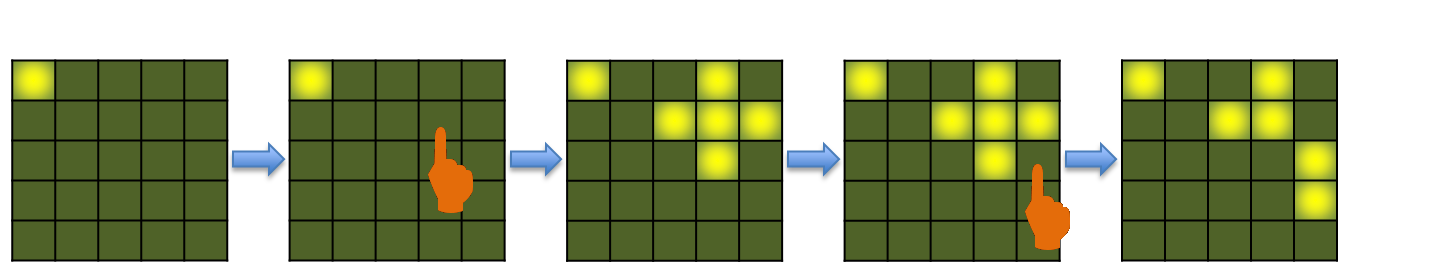
\includegraphics[width=0.9\textwidth]{\img/lightsout.png}
\end{center}
We represent boards as a vector of bits (see Section
\ref{sec:bitarray}). When printing boards in ASCII we represent a
square that is ``on'' (represented by the bit \lstinline'1' or
\lstinline'true') with a `\lstinline"#"' and a square that is ``off''
(represented by the bit \lstinline'0' or \lstinline'false') with a
`\lstinline"O"'. A touch is described by a `row:column pair' as in
previous assignments. On Andrew, we have provided an executable file,
\lstinline'loplayer', that allows you to play Lights Out. The text in
italics below represents the part that you would type in during the above
session.
\begin{quote}
\lstinline'%' \emph{loplayer boards/board0.txt}\\
\lstinline'#OOOO'\\
\lstinline'OOOOO'\\
\lstinline'OOOOO'\\
\lstinline'OOOOO'\\
\lstinline'OOOOO'\\
\emph{1:3}\\
\lstinline'Flipping 1:3'\\
\lstinline'#OO#O'\\
\lstinline'OO###'\\
\lstinline'OOO#O'\\
\lstinline'OOOOO'\\
\lstinline'OOOOO'\\
\emph{2:4}\\
\lstinline'Flipping 2:4'\\
\lstinline'#OO#O'\\
\lstinline'OO##O'\\
\lstinline'OOOO#'\\
\lstinline'OOOO#'\\
\lstinline'OOOOO'
\end{quote}
You can exit \lstinline'loplayer' by typing in something invalid, by
pressing Ctrl-D, or by winning the game and turning all the lights
out.

\clearpage
\section{Bit Vectors}
\label{sec:bitarray}

The \lstinline'pixel' type used a single 32-bit integer to efficiently
store four 8-bit numbers. A single 32-bit integer could, by the same
principle, store up to 32 true/false values. That is what the bit
vector implementation that you will be implementing does. Bit vectors
are an abstraction that assists us in efficiently manipulating small
sequences of bits.  We'll use these sequences of true/false bits to
store the on/off squares in a Lights Out board.

The function \lstinline'bitvector_new()' gives us a fresh bit vector
containing only \lstinline'false' bits, the function
\lstinline'bitvector_get(B, i)' tells us whether the \lstinline'i'th
bit of the vector is true, and the function
\lstinline'bitvector_equal(B1, B2)' returns \lstinline'true' if all
the bits in \lstinline'B1' and \lstinline'B2' are the same. Obviously,
we could implement \lstinline'bitvector_equal' by calling
\lstinline'bitvector_get' in a loop, but we expect that the library
may be able to implement a more efficient equality check.

The function \lstinline'bitvector_flip(B, i)' returns a new bit vector
that is just like \lstinline'B' except that the
\lstinline'i'\textsuperscript{th} bit is flipped.  Unlike C and C0
arrays, bit vectors are a persistent data structure: when we flip a
bit in a bit vector, the old bit vector stays the same and we return a
new bit vector with the bit toggled.

\begin{task}[5]
\TAGS{bit-patterns}
Implement the \lstinline'lib/bitvector.h' interface in a file called
\lstinline'bitvector.c'.
% According to \lstinline'lib/bitvector.h', the type
% \lstinline'bitvector' is defined to be an unsigned integer type with at
% least \lstinline'BITVECTOR_LIMIT' bits in it.
\end{task}

This task is all you need to do in order to successfully begin working
on your Lights Out implementation. However, there are two additional
challenges for your bit vector implementation. First, notice that the
macro-defined constant \lstinline'BITVECTOR_LIMIT' is set to be 25 in
your version of \lstinline'lib/bitvector.h'. Given that the type
\lstinline'bitvector' is a 32-bit unsigned integer, the constant
\lstinline'BITVECTOR_LIMIT' could just as easily be set to 8 or 32
(but not 33 or 42).

\begin{task}[1]
\TAGS{bit-patterns}
  Make your implementation of \lstinline'bitvector.c' work correctly
  regardless of what \lstinline'BITVECTOR_LIMIT' is. You should assume
  that this limit is greater than 0 and less than or equal to the
  number of bits in the type \lstinline'bitvector'.
\end{task}

\bigskip The type \lstinline'bitvector' is defined in
\lstinline'lib/bitvector.h' to be a 32 bit unsigned integer. But if we
need bit vectors of length 33 or 42, it should be possible to use a
larger unsigned integer type, and if we only need bit vectors of
length 7, it should be possible to use a smaller unsigned integer
type.

\begin{task}[2]
\TAGS{bit-patterns, c-numbers}
  Make your implementation of \lstinline'bitvector.c' work correctly
  regardless of what unsigned integer type \lstinline'bitvector' is
  defined to be. You may assume that whatever unsigned integer type
  \lstinline'bitvector' is defined to be has at least
  \lstinline'BITVECTOR_LIMIT' bits in its representation.
\end{task}

\subsection*{Using Bit Vectors}

Remember that, in the pixels assignment, we gave you a separate
implementation of pixels that stored these four numbers in an array
with length 4.  It's similarly possible to use either a 32-bit integer
or a \lstinline'bool' array with length 25 to store 25 true/false
values. Because we are using C, an array implementation would
presumably lead to unrecoverable memory leaks, because we don't expose
a \lstinline'bitvector_free' function.

We will compile your code that uses bit vectors against such other
implementations, including an implementation that is a
\lstinline'bool' array.  Aside from memory leaks, your code for tasks
4-6 should work with these other implementations. In other words, for
the remainder of the assignment, you should respect the
\lstinline'bitvector' interface: you shouldn't assume you know
anything about how a bit vector is implemented.








%% bits. But it could be 64 bits, or 4 bits, or

%% along with the constant
%% \lstinline'BITARRAY_LIMIT' that defines how many true/false values can be
%% stored in a bit array. In \lstinline'lib/bitarray.h', the type
%% \lstinline'bitarray' is defined to be a 32-bit unsigned integer, and
%% \lstinline'BITARRAY_LIMIT' is defined to be 25. However,
%% \lstinline'BITARRAY_LIMIT' could be just as well defined to be 32 or 8,




%% constant

%% The size of a bitarray is defined by the macro \lstinline'BITARRAY_LIMIT'.

%%  use either arrays of type \lstinline'bool' to store
%% a number of true/false values.


%% The bit array interface file \lstinline'lib/bitarray.h' constrains \emph{both}
%% the client and the library. The interface specifies that bit
%% arrays must be unsigned integer types, and that these unsigned
%% integers must contain at least \lstinline'BITARRAY_LIMIT' bits.
%% %% The
%% %% quantity \lstinline'BITARRAY_LIMIT' is defined to be 25 in your
%% %% \lstinline'lib/bitarray.h', but if that quantity changes your
%% %% implementation of bit arrays and your implementation of Lights Out
%% %% should still work assuming that the \lstinline'bitarray' type has at least
%% %% \lstinline'BITARRAY_LIMIT' bits.

%% When you are acting as the implementer of bit arrays by writing
%% \lstinline'bitarray.c', respecting the interface means that you can't
%% assume you know precisely what type a \lstinline'bitarray' is. The type
%% \lstinline'bitarray' is defined in \lstinline'lib/bitarray.h', and your
%% implementation in \lstinline'bitarray.c' should assume only that this type
%% is defined to be an unsigned integer type that contains at least
%% \lstinline'BITARRAY_LIMIT' bits. The \lstinline'lib/bitarray.h' interface could
%% change to define \lstinline'bitarray' as another type and/or define
%% \lstinline'BITARRAY_LIMIT' to be a different positive number, and your
%% bitarray implementation should still work. Because it might be
%% undefined behavior to shift by more than \lstinline'BITARRAY_LIMIT' bits,
%% your contracts will have to mention this macro-defined constant.

%% When you are acting as the client of bit arrays, respecting the
%% interface means using \lstinline'BITARRAY_LIMIT' instead of assuming that
%% its value is 25, 32, 8, or some other constant.\footnote{The
%%   \texttt{file\_read} function we give you in \texttt{lib/boardutil.h}
%%   uses \texttt{BITARRAY\_LIMIT} to fail if your Lights Out board is
%%   too big to fit in a \texttt{bitarray}.} It also means \emph{only}
%% using \lstinline'bitarray_new' to get an empty bitarray and \emph{only}
%% using \lstinline'bitarray_get' and \lstinline'bitarray_flip' to access individual
%% bits in the bit array. We will compile your Lights Out implementation
%% against bit array implementations that store bits in a different order
%% than your implementation stores them. We will even compile
%% your Lights Out implementation against bit array implementations where
%% \lstinline'bitarray_new()' does not return \lstinline'0'. (Your
%% implementation should probably return \lstinline'0'.)\footnote{A puzzle to
%%   think about: how could you implement the bitarray interface if
%%   \texttt{bitarray\_new} returned \texttt{\textasciitilde{0}} instead
%%   of the obvious value of \texttt{0} that your implementation will
%%   probably use?}  Your code that uses bitarrays must work even when
%% given these strange implementations.

%% Clients \emph{can} compare bit
%% arrays \lstinline'B1' and \lstinline'B2' for equality using \lstinline'B1 == B2', and
%% they can cast bitarrays to the unsigned type \lstinline'size_t' and perform
%% mathematical operations to the result. Both of these will be useful
%% when you need to store bit arrays as the keys to a hashtable. (If it
%% happens that \lstinline'BITARRAY_LIMIT' is larger than the number of bits
%% in a \lstinline'size_t', then the cast from \lstinline'bitarray' to
%% \lstinline'size_t' would truncate the bitarray to make it fit. This is not
%% something you need to worry about here: even if it happened, it
%% wouldn't be the end of the world for a hash function to behave this
%% way.)

%% Our implementation of the \lstinline'lib/boardutil.h' library function
%% \lstinline'file_read' checks that the board being read from a file has no
%% more than \lstinline'BITARRAY_LIMIT' bits, so this part of the client's
%% responsibility is handled for you.


\section{Hash Tables}

The algorithm we describe for solving Lights Out is going to use hash
tables which will store Lights Out boards that have already been
looked at --- this prevents you from doing computation for them again.
We provide you with the generic version of automatically-resizing,
separate-chaining hash dictionaries as described in
\lstinline'lib/hdict.h' --- you do \emph{not} have to implement hash
tables from scratch.

However, instantiating the client interface and casting void pointers
correctly in C is error-prone. For this task, you will implement, in
\lstinline'board-ht.h' and \lstinline'board-ht.c', a wrapper around
the \lstinline'hdict' interface that handles the tricky parts.

Specifically, the functions you will have to implement are:

\begin{itemize}
\item%
  \lstinline'ht_new', which creates a new, initially empty, hashtable
  and correctly instantiates the client interface.
\item%
  \lstinline'ht_insert', which adds a new %
  \lstinline'struct board_data' %
  to the table.
\item%
  \lstinline'ht_lookup', which looks up structs in the hash table
  based on the key, a \lstinline'bitvector' stored in the
  \lstinline'board' field of the struct.
\end{itemize}

When the \lstinline'ht_insert' function is given a %
\lstinline'struct board_data DAT', %
it needs to perform an insertion into the hash table using
\lstinline'hdict_insert'. The \textbf{entry} stored in the hash table
should be a pointer to the \lstinline'struct board_data DAT' that is
passed to \lstinline'ht_insert'.  The \textbf{key} of this entry
should be a pointer to the \lstinline'board' bitvector of the
underlying struct; you'll need to take the address of
\lstinline'DAT->board' to get this pointer.

There is no \lstinline'ht_free' because it would work the same way as
the free function provided by the \lstinline'hdict' interface. Pointers
added to the hash table with \lstinline'ht_insert' are owned by the
table, and should be freed when \lstinline'hdict_free' is called

\begin{task}[6]
\TAGS{dictionary, genericity, hashing}
Implement the \lstinline'board-ht.h' interface in a file called
\lstinline'board-ht.c'.
\end{task}

You're not required to use these hash tables in your Lights Out
implementation, but we certainly suggest you do!  Whether you use them or
not, your implementation of the interface will be autograded. The
elements in the hash table are pointers to \lstinline'struct board_data', a
struct with two fields.

\emph{You can edit \lstinline'board-ht.h' to add any fields that
  you want to the \lstinline'struct board_data', but the autograder
  will require that the original two fields remain the first two
  fields in the struct.}


\clearpage
\section{Lights Out}

In this section, you will implement a solver that can decide whether
or not a board is solvable, and that describes how to solve boards
that can be solved.

A reference solution, which is about as efficient as your solution
needs to be, can be found on Andrew with the name
\lstinline'lightsout-ref'.

\begin{lstlisting}[language={[coin]C}, deletestring={[b]{'}}]
% lightsout-ref boards/3x2-34.txt
Here's the board we're starting with:
#OO
##O

Board is solvable.
Solution bitmap (the squares marked # need to be pushed to solve):
OOO
#OO

% lightsout-ref boards/3x2-32.txt
Here's the board we're starting with:
#O#
#OO

No solution was found!
\end{lstlisting}

Your implementation of a solver for Lights Out in
\lstinline'lightsout.c' should produce an executable that takes one
command-line argument, the filename of a file containing a board which
can be read with the \lstinline'file_read' function from
\lstinline'lib/boardutil.h'. \textbf{The output from your solver will
  be a bit different than the output from the reference solution; read
  the instructions carefully.}

To take command-line arguments in C, you need to write a
\lstinline'main' function with two arguments, \lstinline'argc'
(\emph{argument count}, the number of command-line arguments) and
\lstinline'argv' (\emph{argument values} an array of strings, the
actual command-line arguments). Our implementation begins like this:

\begin{quote}
\begin{lstlisting}[numbers=none]
int main(int argc, char **argv) {
  if (argc != 2) {
    fprintf(stderr, "Usage: lightsout <board name>\n");
    return 1;
  }
  char *board_filename = argv[1];
  ...
}
\end{lstlisting}
\end{quote}

If you want to print out debugging information or error messages in
your implementation, you should use \lstinline'fprintf(stderr,...)'
instead of \lstinline'printf(...)' the way we do above. Do not use
\lstinline'printf'.  Using \lstinline'fprintf(stder,...)' ensures that
all error messages or debugging outputs go to \emph{standard error},
which will be critical for Task 6. (Output from failed contracts
automatically goes to standard error.)


\subsection{Solving Lights Out}

The return value of \lstinline'main' in a C program is treated as
meaningful to the operating system. Returning 0 means the program ran
successfully and returning anything else means the program ran
unsuccessfully. For your Lights Out solver, the \lstinline'main()'
function in your implementation must return \lstinline'0' if the board
can be solved, and should return \lstinline'1' if there was an error
\textbf{or} if the Lights Out board cannot be solved. A C program will
not print out the returned integer like a C0 program does, so you
probably want to print a helpful ``board could be solved'' or ``board
could not be solved'' message to standard error.

\begin{task}[6]
\TAGS{c-memory, c-numbers, complexity, ds-traversal, search}
  Implement a Lights Out solver in \lstinline'lightsout.c' that takes
  a board and reports whether or not the board is solvable by
  returning \lstinline'1' or \lstinline'0' from the \lstinline'main()'
  function.
\end{task}

Any valid implementation of Lights Out with reasonable performance
will get points. You're welcome to be creative, but any creative idea
you implement should be your own. (There are academic papers on the
mathematics of Lights Out and its solutions, including a 1989 paper by
the computer science department's own Klaus Sutner! But for this
assignment, if you do something different than the strategy outlined
in this writeup, it should be your own idea.) We suggest that you
first implement the \emph{breadth-first search} algorithm outlined in
Section \ref{sec:bfs}.  But if you want a challenge, you're encouraged
to try and figure out an algorithm on your own.

Your implementation should be free of memory leaks (as reported by
\lstinline'valgrind') \emph{regardless} of whether your
\lstinline'main' function returns \lstinline'0' or \lstinline'1'. Your
implementation should also work regardless of the way bit vectors are
implemented.

For this assignment, we have given you a \lstinline'Makefile' to help
you build your solver. If you type \lstinline'make' after writing
\lstinline'bitvector.c', \lstinline'board-ht.c', and
\lstinline'lightsout.c' it will compile two executables,
\lstinline'lightsout' and \lstinline'lightsout-d' (the latter is
compiled with \lstinline'-DDEBUG'). You can change your Makefile to
add new targets (for instance, to run unit tests for your bit
vectors).


\subsection{Returning the Solution}

\begin{task}[5]
\TAGS{c-memory, c-numbers, complexity, ds-traversal, search}
  Modify your Lights Out solver so that, when it is given a solvable
  board, it prints out, to standard output, the series of button
  pushes that solve the board.
\end{task}

The output of your program should not be like the reference solution's
output. Instead, if a solution is found, all the moves leading to that
solution should be printed, in order, to \emph{standard output} (or
\lstinline'stdout', which is what \lstinline'printf' prints to). The
output should be able to be re-routed into \lstinline'loplayer' as
input that solves the board. See Section~\ref{sec:testing} for an
example. (If no solution is found, nothing should be printed to the
standard output, and it's a good idea to print ``No solution'' to
\lstinline'stderr'.)

% A challenge for this assignment will be figuring out what data you
% need to store in your queue and what data you need to store in your
% hash table. However you do it, once you find a winning solution, you
% must also recover the moves you used to get to that board. You may want
% to add fields to \lstinline'struct board_data' to do this task.

You may want to add fields to \lstinline'struct board_data' to do this
task.

% ???
An examination of the puzzle leads to interesting observations ---
changing the state of a square an even number of times is equivalent
to not changing it at all; changing the state an odd number of times
is equivalent to changing it only once. Furthermore, the order in
which we touch various squares is unimportant. It is only the number
of times that we touch a square that matters. These facts imply that,
if a puzzle can be solved at all, it can be solved by touching some
squares exactly once and others not at all. Thus, a solution consists
of indicating which squares to touch once.

Therefore, one way to complete this task is to store boards in the
hash table alongside a bit vector representing \emph{all} the moves
needed to produce that board. Another option is to store boards along
with the index of the move that got you to that board. Then you can
find the solution by working backwards. When you notice you have a
board with all lights out, re-apply the last move to get the previous
board. Then look up that previous board in the hashtable, which will
also give you the move that allowed you to reach \emph{that} board,
and so on and so forth until you get back to your original board.



\subsection{Testing}
\label{sec:testing}

You'll want to be sure to test your solver on boards that aren't
symmetric and examples that aren't squares. A good way to test your
program is to use a Unix \emph{pipe}, redirecting the standard output
of your Lights Out solver to the standard input of the
\lstinline'loplayer' program:

\begin{quote}
\begin{lstlisting}[language={[coin]C}]
% ./lightsout boards/3x2-34.txt
1:0
% ./lightsout boards/3x2-34.txt | loplayer boards/3x2-34.txt
#OO
##O
Flipping 1:0
OOO
OOO
You got all the lights out!
\end{lstlisting}
\end{quote}

When testing your solution on the boards we provide, be aware that if
you have good contracts, your code may be too slow to solve the harder
boards in reasonable time. Once you are confident of the correctness
of your code, run your tests on \lstinline'./lightsout', not
\lstinline'./lightsout-d'.

Every 2x2 board and an assortment of 3x2 and 4x4 boards are
distributed with the handout. \textbf{When compiled without -D,} your
solution should be able to solve all the 2x2 boards (or report no
solution) instantly and do the same for any 3x2 and 4x4 board in
seconds at most. The included 5x5 boards may be too challenging for
your implementation, but you should be able to search any 5x5 board
that takes less than 6 touches to finish without much difficulty.
\emph{You can share test boards and solutions to individual boards on
  \qatool{}.}

\clearpage
\subsection{Suggested Algorithm: Breadth-First Search}
\label{sec:bfs}

The algorithm we will sketch out here for solving Lights Out is called
\emph{breadth-first search}.  The basic version of breadth-first
search uses a queue. We start with just the initial board in the
queue, and then we begin a loop. As long as the queue is not empty,
one iteration of the loop removes a board from a queue, computes the
effect that each of the 25 possible button-pushes will have on the
board, and then inserts all 25 modified boards back onto the queue. If
we do this very naively, the algorithm will first consider the one
board that we can get to with zero touches, then the 25 boards we can get
to with one touch, then the 625 boards we can get to with two touches,
then the 15,625 boards we can get to with three touches, and so on.

This approach will always find a solution if one exists, but it is
very wasteful, because we can get to the rightmost board on
page~\pageref{sec:intro} in two different ways: by touching the square
in row 1, column 3 and then the square in row 2, column 4 and also by
touching the square in row 2, column 4 and then by touching the square
in row 1, column 3.  The naive algorithm described in the previous
paragraph unnecessarily considers both of these possibilities
separately.

We solve the problem more efficiently with a hash table. When we start
the loop, the initial board is also present in the hash table. Inside
the loop, we can compute all 25 possible moves but we \emph{only}
enqueue and add to the hash table the ones that we haven't previously
considered. Here is pseudocode for the resulting algorithm:

\medskip
\begin{lstlisting}[language={[coin]C}, deletestring={[b]{'}}]
while (!queue_empty(Q)) {
   // Find a board that we haven't looked at yet from the queue
   B = deq(Q);

   // Consider all the moves
   for (row = 0; row < height; row++) {
      for (col = 0; col < width; col++) {
         i = get_index(row, col, width, height);
         bitvector newboard = press_button($\emph{...}$)

         if ($\emph{number of lights of newboard}$ == 0) {
            $\emph{Free all memory}$, return 0
         }

         if ($\emph{hash table H doesn't contain newboard}$) {
            $\emph{Allocate memory for hashtable element N}$
            $\emph{Set the field N->board to newboard, set other fields}$
            $\emph{Insert N into the hashtable H}$
            $\emph{Enqueue N into the queue Q}$
         }
      }
   }
}
$\emph{Free all memory}$, return 1
\end{lstlisting}


\end{document}
